\documentclass[11pt]{article}
\usepackage{graphicx}

      \textwidth 15cm
      \textheight 22cm
      \parindent 10pt
      \oddsidemargin 0.85cm
      \evensidemargin 0.37cm
      
\usepackage{enumerate}
\usepackage{amsmath}
\usepackage{booktabs} % For pretty tables
\usepackage{caption} % For caption spacing
\usepackage{subcaption} % For sub-figures
\usepackage{graphicx}
\usepackage{float}
\restylefloat{table}
\usepackage[export]{adjustbox}\
\usepackage{pgfplots}
\usepackage[all]{nowidow}
\usepackage[utf8]{inputenc}
\usepackage[english]{babel}
\usepackage[sorting=none]{biblatex}
\addbibresource{references.bib}
\usepackage{csquotes}
\usepackage{tikz}
\usetikzlibrary{er,positioning,bayesnet}
\usepackage{multicol}
\usepackage{algpseudocode,algorithm,algorithmicx}
\usepackage{minted}
\usepackage{hyperref}
\usepackage[inline]{enumitem} % Horizontal lists
\usepackage{listings}
\usepackage{multirow}
% Used for displaying a sample figure. If possible, figure files should
% be included in EPS format.
%
% If you use the hyperref package, please uncomment the line
% to display URLs in blue roman font according to Springer's eBook style:
% \renewcommand\UrlFont{\color{blue}\rmfamily}

\newcommand{\card}[1]{\left\vert{#1}\right\vert}

\makeatletter
\newcommand\ackname{Acknowledgements}
\if@titlepage
   \newenvironment{acknowledgements}{%
       \titlepage
       \null\vfil
       \@beginparpenalty\@lowpenalty
       \begin{center}%
         \bfseries \ackname
         \@endparpenalty\@M
       \end{center}}%
      {\par\vfil\null\endtitlepage}
\else
   \newenvironment{acknowledgements}{%
       \if@twocolumn
         \section*{\abstractname}%
       \else
         \small
         \begin{center}%
           {\bfseries \ackname\vspace{-.5em}\vspace{\z@}}%
         \end{center}%
         \quotation
       \fi}
       {\if@twocolumn\else\endquotation\fi}
\fi
\makeatother
\pgfplotsset{compat=1.16}

\begin{document}

\thispagestyle{empty}


\begin{center}

Vrije Universiteit Amsterdam

\vspace{1mm}


\includegraphics[height=28mm]{VUlogo_NL_Wit_HR_RGB_tcm289-201376.png}

\vspace{1.5cm}

{\Large Bachelor Thesis}

\vspace*{1.5cm}

\rule{.9\linewidth}{.6pt}\\[0.4cm]
{\huge \bfseries Benefits of data scalabilty and transfer learning for relational graph data\linebreak (Machine learning - RGCN, scalability)\par}
\vspace{0.4cm}
\rule{.9\linewidth}{.6pt}\\[1.5cm]

\vspace*{2mm}

{\Large
\begin{tabular}{l}
{\bf Author:} ~~Karim Anwar ~~~~ (2615855)
\end{tabular}
}

\vspace*{1.5cm}

\begin{tabular}{ll}
{\it 1st supervisor:}   & ~~Michael Cochez \\
{\it daily supervisor:} & ~~Michael Cochez \\
{\it 2nd reader:}       & ~~Daniel Daza
\end{tabular}



\vspace*{2cm}

\textit{A thesis submitted in fulfillment of the requirements for\\ the VU Bachelor of Science degree in Computer Science }

\vspace*{1cm}

\today\\[4cm] % Date

\end{center}

\newpage



% \twocolumn




\begin{abstract} \textbf{The goal of this paper is to present a framework that tackles the issue of data scalability for graph data. This framework is split into two parts, the first part consists of data summarization which consist of making new graph by learning the connections done between node types which decreases the amount of memory needed especially that GPUs, even now that they are faster, are still, not match for CPUs when it comes to space and the learning time needed for the model will decrease as well. In the second part, transfer learning will be used to introduce the knowledge of one model to another with the original datasets, the parameters of first model which will decrease the time needed to train, which will increase overall speed gain in the learning process.}
\end{abstract}


\section{Introduction} The recent success of convolutional  neural networks (CNN) and deep learning in many domains is due to the rapidly developing computational resources (eg.GPU), and the availability of big training data (eg.Knowledge Bases), and the effectiveness of deep learning to extract latent representations. While deep learning effectively captures hidden patterns from Euclidean data, there is an increasing number of applications where the data is represented in the forms of graphs. From citation networks, which shows how papers are linked to each other, to medical fields with representations of interactions between molecules which each represent a different graph. A new family of networks called graph neural networks (GNN) come to existence with how graph data became ubiquitous in the Machine learning community. With the introduction of Graph Convolutional Networks (GCN) \cite{kipf2016semi} which generalizes  GNNs, learning can not be simpler than it is today. Knowledge Bases are growing at an explosive rate, and the same goes for the number of missing data in them. Ontologies like RDF and OWL not only have they simplified the representation of these KBs, but they have also provided a common framework so data can be exchanged between applications without loss of meaning. RDF use a format of triples which presents the relationship between two nodes, a subject, an object, and a predicate that links them, to tackle this new data Relational Graph Convolutional Network (RGCN) \cite{schlichtkrull2017modeling} had to be introduced which took in consideration the information that resides on the edges (relationships) of the graph. This makes the data richer, but also increases their complexity: the size of the data makes it difficult to train on it, as it is not obvious to scale it without losing information, because this is where the biggest problem of graph data resides.
This paper is organised as following:
In Section 2, we provide the essential concepts that will be presented throughout the paper. In Section 3 we introduce the main methods used in the paper that address the topic of scalability and in section 4 the ones of transfer learning. We provide our analysis and insights in Section 5, in section a brief discussion comparing our results to other papers, and the conclusion in Section 6.


\section{Preliminaries}\label{ref:prelim}
In this section, we will recall some key concepts, in this paper we will consider a directed and labeled multi-graph as  $G = (\mathcal{V}, \mathcal{E}, \mathcal{R})$ with nodes (entities) $v_i \in \mathcal{V}$ and labeled edges (relations) $(v_i, r, v_j) \in \mathcal{E}$, where $r\in\mathcal{R}$ is a relation type.

\subsection{Relational graph convolutional networks}
Introduced first as an GCN by Kipf and Welling \cite{kipf2016semi} as a method to generalize graph data analysis where a layer has the form: 

\begin{equation}
\label{eq:gcn_layer}
    h^{(l+1)}_{v_i} = \sigma \left( \sum_{j} \frac{1}{c_{ij}}h^{(l)}_{v_j}W^{(l)} \right),
\end{equation}

where j indexes the neighboring nodes of vi. cij is a normalization constant for the edge (vi,vj) which originates from using the symmetrically normalized adjacency matrix ${D^{-\frac{1}{2}}AD^{-\frac{1}{2}}}$ which then gets used as an extension for large scale relational data, which modifies the forward pass equation:

\begin{equation}
\label{eq:rgcn_layer}
    h_i^{(l+1)}= \sigma \left( \sum_{r \in \mathcal{R}}\sum_{j \in \mathcal{N}^r_i} \frac{1}{c_{i,r}}W_r^{(l)} h_j^{(l)} + W_0^{(l)}h_i^{(l)} \right),
\end{equation}
 where $\mathcal{N}^r_i$ denotes the set of neighbor indices of node $i$ under relation $r\in\mathcal{R}$. Different from regular GCNs, relation specific transformation gets introduced to take in count the information on the graph edges.
 
\subsection{Graph Autoencoders (GAE)}
Recently graph autoencoders \cite{kipf2016semi} and variational graph autoencoders \cite{kipf2016variational} have emerged as powerful models that showed remarkable result for (semi-)supervised and unsupervised learning to learn the graph data characteristics, the proceed by mapping (encoding) the node and edge features of the graph to a low dimensional vector to be able to capture and reconstruct the graph structure which is crucial for the data scalibilty \cite{EmbedingScalability}. In basis the point of using GAE is to be able to reconstruct $A$ from $Z$, where $A$ is the adjacency matrix and $Z$ is the $n \times f$ matrix of all latent space vectors is the output of a Graph Neural Network (GNN) with $\hat{A}$ the reconstruction of the adjacency matrix:

\begin{equation}
\hat{A} = \sigma(ZZ^T) \hspace{10pt} \text{with} \hspace{10pt} Z = \text{GNN(X,A)}.
\end{equation}


\subsection{Entity classification}
 Entity classification for graph data is a RGCN classifier where its layers  \eqref{eq:rgcn_layer}, where it has a minimum of 2 layers, the classifier takes the nodes representations and predicts the labels, the model is learned by minimizing the cross-entropy loss:

\begin{equation}
\mathcal{L}= -\sum_{i\in\mathcal{Y}}\sum_{k=1}^K t_{ik} \ln h_{ik}^{(L)}  \, ,
\label{eq:loss}
\end{equation} 

where $\mathcal{Y}$ is the set of node indices that have labels and $h_{ik}^{(L)}$ is the $k$-th entry of the network output for the $i$-th labeled node. $t_{ik}$ denotes its respective ground truth label. 

\section{Graph scalability}
In this section, we introduce the concept of querying and summarizing graphs used for the experiment. 

\subsection{Graph summarization}
Data summarisation when applied to machine learning has a fine line between time performance and results accuracy, having the data in RDF is a plus when we want to have the data summarized, a paper like "Summarizing Semantic Graphs: A Survey" \cite{Cebiric2019} shows a collection of methods by different researchers on RDF summarization, some specific papers like "Simplifying RDF Data for Graph-Based Machine Learning" \cite{Bloeam2014simplifrdf} which shows remarkable performance when it comes to RDF summarization and "A Degeneracy Framework for Scalable Graph Autoencoders" \cite{salha2019degeneracy} which presents results for speed performance and accuracy performance using graph auto-encoders and GCNs, but the paper that inspired our framework is "Graph Summarisation of Web Data: Data-driven Generation of Structured Representations"\cite{Campinas2016GraphSO} which utilises SPARQL queering to obtain results via bi-simulation, where our framework uses the same queering method to summarize the data by node type to get a summary on the node collection layer of the original data \cite{6327436}.

\subsection{Type summarization}
The Resource Description Framework (RDF) s a simple format of triples which is composed of subjects, predicates, and objects, where each unique node from the collection of the subjects and objects combined represents and actual node from the data graph. Using SPARQL as querying language RDF schema can be filtered out to get from it the types of the nodes, which these types then will become the main nodes of the summarized graph, and what happens in the SPARQL query is that a PREFIX line is put in place to recognize the types and from the extracted unique subject and object types a new graph is constructed which keeps the relationships between the original nodes that becomes the relationship between the "Type" nodes of the new graph. Accordingly, the size of the the original graph will be greatly reduced depending on the diversity of the nodes types in it upon which that diversity will determine the size of the new reduced graph.

\begin{figure}[H]
    \centering
    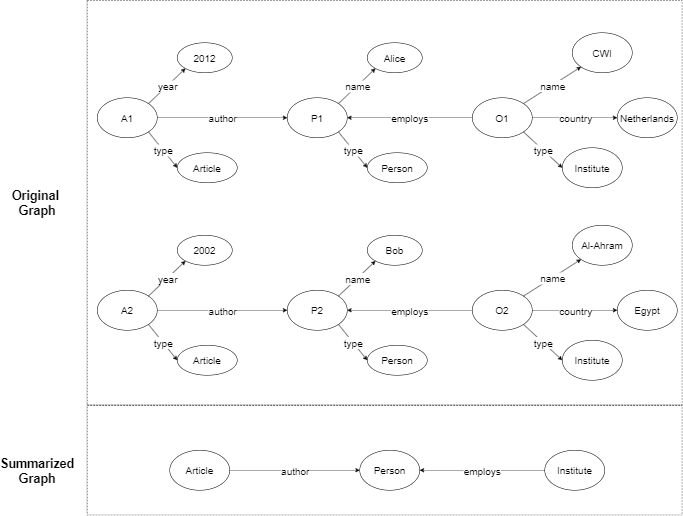
\includegraphics[width=0.8\linewidth, frame]{new_diag.png}
    \caption{\small An example of type summarization}
    \label{fig:type_summary}
\end{figure}

\section{Transfer learning}
The basic idea of transfer learning is to use knowledge learned from a previous source domain to improve the performance of the learned decision functions of the target domain according to the definition in \cite{zhuang2019comprehensive}. Transfer learning is really useful to not reduce training time and gain remarkable results from our model by using the best trained parameters learned from another model, a variety of pre-trained neural networks exist which were trained on a vast amount of data. The ImageNet project for image classification, for example, is one of these pre-trained models which has 14 million images which belong to more than 20,000 classes. All the parameters learned from the source model that was trained on a prior time can be transferred to the target model to gain valuable time and resources, but some criteria still have to be taken into consideration, the similarity of the datasets as well as their size. The most common case of transfer learning of a new dataset is when said dataset is smaller than the original and they are both similar so to avoid overfitting when training the classifying layer is the only layer to be fine-tuned. Another form of transfer learning is when the new dataset is larger than the one of the pre-trained model. In this latter case, we would have more confidence in not overfitting and we could fine-tune through the entire network.

\begin{figure}[H]
    \centering
    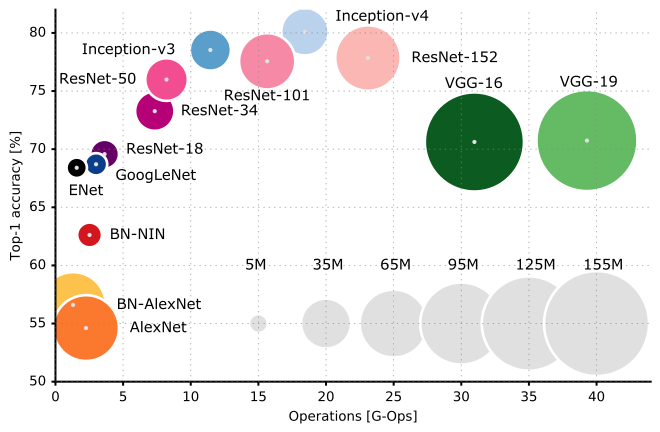
\includegraphics[width=0.8\linewidth, frame]{tl.png}
    \caption{\small Collection of public NN models, on a scale of the  accuracy achieved upon conception, with respect to the dataset size used for training}
    \label{fig:pre_trained}
\end{figure}

\subsection{Inductive transfer learning}
 Inductive transfer learning is a form of transfer learning for where the target task is different from the source task, regardless of whether the source and target domains are identical or not \cite{Pan2010ASO}.
 Inductive learning can be categorized into two cases:
 \begin{enumerate}[label=\alph*.]
     \item  There is a lot of labeled data in the source domain. The inductive transfer learning setting is analogous to the multitask learning environment in this scenario. Inductive transfer learning, on the other hand, focuses solely on improving performance in the target task by transferring knowledge from the source task, whereas multitask learning tries to learn both the target and source tasks at the same time.
     \item No labeled data in the source domain are available. In this case, the inductive transfer learning setting is similar to the self-taught learning setting. In the self-taught learning setting, the label spaces between the source and target domains may be different, which implies the side information of the source domain cannot be used directly. Thus, it’s similar to the inductive transfer learning setting where the labeled data in the source domain are unavailable.
 \end{enumerate}
 Which then is used to apply an approach referred to as feature-representation-transfer approach an example of that is represented the paper of Blitzer et al. \cite{blitzer-etal-2007-biographies}. The intuitive idea behind this case is to learn a “good” feature representation for the target domain. In this case, the knowledge used to transfer across domains is encoded into the learned feature representation. With the new feature representation, the performance of the target task is expected to improve significantly.


 \begin{figure}[H]
    \centering
    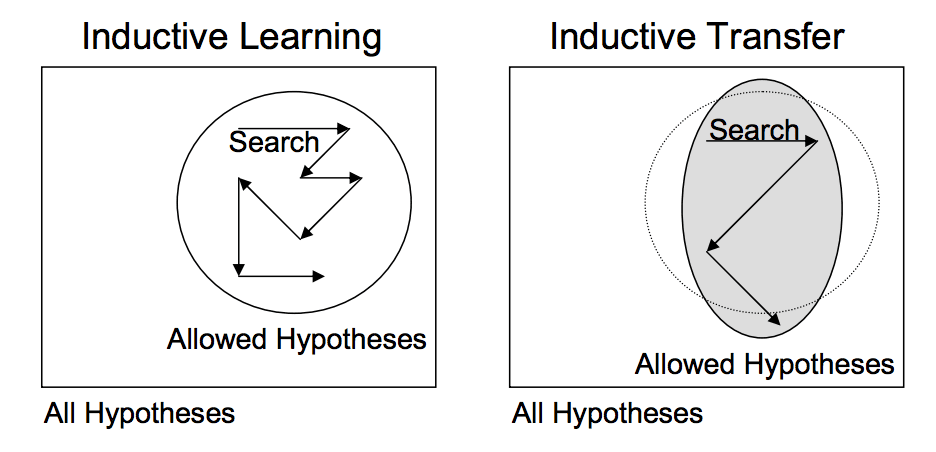
\includegraphics[width=0.8\linewidth, frame]{inductive transfer.png}
    \caption{\small Comparison between Inductive learning and Inductive transfer learning}
    \label{fig:pre_trained}
\end{figure}


\subsection{How transferable are the features?}
If the target dataset is small and the number of parameters is large, fine-tuning may result in overfitting, so the features are often left frozen. On the other hand, if the target dataset is large or the number of parameters is small, so that overfitting is not a problem, then the base features can be fine-tuned to the new task to improve performance. Of course, if the target dataset is very large, there would be little need to transfer because the lower level filters could just be learned from scratch on the target dataset. \cite{yosinski2014transferable}
Typically in transfer learning the new dataset is larger and similar to the original dataset which prevents overfitting when trying to fine-tune through the full network.
In other cases the new dataset is large and very different from the original. Since the dataset is very large, we  may expect that we can afford to train a convolutional network from scratch. In practice, though, it is often still beneficial to start with weights from a trained model. We'd have enough data and confidence in this case to fine-tune the network as a whole.\\* However, for our problem the new dataset is small and different from the original, it is likely best to only train a linear classifier. Since the dataset is very different, it may not be optimal to train the classifier using the network's top layer, which contains more dataset-specific features. Instead, it might work better to train the classifier from activations somewhere earlier in the network.



\section{Empirical evaluation}
In this section, we empirically evaluate our model combined with our introduced framework.

\subsection{Experimental Setting}
\paragraph{Datasets}
We evaluate our model on four datasets\footnote{https://github.com/rusty1s/pytorch\_geometric/blob/master/torch\_geometric/datasets/entities.py} in RDF format: AIFB, MUTAG, BGS, and AM. The AIFB dataset describes the AIFB research institute in terms of its staff, research group, and publications. The dataset was first used to predict the affiliation (i.e., research group) for people in the dataset. The dataset contains 178 members of a research group, however the smallest group contains only 4 people, so this one is removed from the dataset, leaving 4 classes. Moreover, we also remove the employees relation, which is the inverse of the affiliation relation from the dataset.The MUTAG dataset contains information about complex molecules that are potentially carcinogenic, which is given by the isMutagenic property. The BGS dataset was created by the British Geological Survey and describes geological measurements in Great Britain. The dataset contains around 150 named rock units with a lithogenesis, from which we used the two largest classes. The AM dataset contains information about artifacts in the Amsterdam Museum. Each artifact in the dataset is linked to other artifacts and details about its production, material, and content. It also
has an artifact category, which serves as a prediction target. We have drawn a stratified random sample of 1,000 instances from the complete dataset. We also removed the material relation, since it highly correlates with the artifact category. And for each of these datasets we use their node type summarized counterparts for transfer task.
\\
\begin{table}[htp!]
\centering
\begin{tabular}{lrrrr}
\toprule
Dataset & AIFB & MUTAG & BGS & AM  \\ \midrule
Entities    & 8,285 & 23,644 & 333,845 & 1,666,764 \\
Relations   & 45 & 23 & 103 & 133 \\
Edges   & 29,043 & 74,227 & 916,199& 5,988,321 \\
Labeled  & 176 & 340 & 146 &  1,000 \\
Classes  & 4 & 2 & 2 &  11 \\

 \bottomrule
\end{tabular}
\caption{Number of entities, relations, edges and classes along with the number of labeled entities for each of the datasets. \textit{Labeled} denotes the subset of entities that have labels and that are to be classified.}
\label{table:classification_datasets}
\end{table}

\paragraph{Task}
We consider the task of entity classification as briefly introduced in section \ref{ref:prelim} where the model acts as a classifier for the entities of the graph to find their corresponding labels which are the node types. Implementing the steps from Schlichtkrull et al. \cite{schlichtkrull2017modeling} with a split of 80/20 of the dataset without a validation set, we can directly extract the hyperparameters from the paper and apply it to the model directly. We track the training time (wall-clock time) of the training of the complete datasets, then we apply transfer learning to use the parameters of a pre-trained model which in this case, is a model we train on a different dataset.

\\
\begin{table}[htp!]
\centering
\begin{tabular}{lrrrr}
\toprule
 & AIFB & MUTAG & BGS & AM  \\ \midrule
Test accuracy    &  94.02 & 70.58 & 81.46 & OOM \\
Training time   & 16s & 11s & 5min53s & OOM \\

 \bottomrule
\end{tabular}
\caption{Training time on the original graphs and the test accuracy results.}
\label{table:training_time}
\end{table}

\paragraph{Model}
The original model has been based on the experiments done in the RGCN modeling paper \cite{schlichtkrull2017modeling}, the RGCN is a basic two-layer classification networking \eqref{eq:rgcn_layer}. The model is trained on 50 epochs, and the training accuracy is averaged for 10 runs. The model\footnote{https://github.com/Karim-Anwar/thesis/} is built using Python, with the usage of Pytorch and Pytorch Geometric libraries to utilize the GPU which has, as specifications, 12.69GB of memory. The training and evaluation was done in the Google COLAB\footnote{https://colab.research.google.com/} environment. The summarization of the graph was done using Java code run over a Intel Core i7 QuadCore CPU. All data summarized was reshaped by padding the tensor manually to have the same shape as the layer we need to fine tune for the transfer learning

\subsection{Results}

As presented before, the training results are in comparison to what other frameworks achieved. In table 3 is the information that will be used as base of comparison from the summarized versions of the graphs and table 4 are the results we got from the transfer learning.

\\
\begin{table}[htp!]
    \centering
    \begin{tabular}{lrrrr}
    \toprule
    Dataset & AIFB & MUTAG & BGS & AM  \\ \midrule
    Original size(in MB)    & 5.95 & 10.2 & 209 & 755 \\
    Summarized size (in KB)  & 26 & 44.1 & 5.94 & 7.79 \\
    Reduction of & 22884\% & 23129\% & 3518518\% & 9691912\% \\
    Summarization time & 3s & 3s & 2min5s & 1min57s \\
    Number of nodes & 26 & 112 & 4 & 20 \\
    Number of edges & 188 & 316 & 41 & 56 \\
     \bottomrule
    \end{tabular}
    \caption{Measured time for type summary and the new size of the dataset memory wise.}
    \label{table:summarization_details}
\end{table}

\\
\begin{table}[htp]
\begin{tabular}{cccccc}
\hline
                                                                                           &          & AIFB  & MUTAG & BGS & AM    \\ \hline
\multirow{2}{*}{\begin{tabular}[c]{@{}c@{}}Save Model from\\ Summarized Data\end{tabular}} & Test Accuracy & 1.6   & 36.89 & 64.66   & 41.14 \\ \cline{2-6} 
                                      & Training Time & 5s & 2s & 8s & 12s   \\ \hline
\multirow{2}{*}{\begin{tabular}[c]{@{}c@{}}Model with Transfer\\ Learning\end{tabular}}    & Test Accuracy & 48.50 & 66.08 & 65.37   & OOM   \\ \cline{2-6} 
                                                                    & Training Time & 13s   & 9s & 3min58s & OOM   \\ \hline
\end{tabular}
\caption{Training time on the summarized graphs and the test accuracy results as well as the their performances after transfer learning.}
\label{table:training_time}
\end{table}

We observe a few interesting things about our results in table 4, we first notice slight to no improvement for the time to train both our model to transfer and our original with that model for the smaller datasets, which were the ones with largest summarized counter parts (AIFB, MUTAG). For the dataset BGS the transfer learning had the opposite effect, where the summary was smaller and more general, had a decrease on the training time from 5 minutes 53 seconds to 2 minutes 58 seconds. While for AM, the training on the target model still went Out Of Memory, but something we noticed is that training on the summarized was possible.\\
None of the three successful model had progress for test accuracy but the datasets from the original lowest had a higher test accuracy compared to the AIFB dataset model.\\
A couple of elements can be observed, first the model with greater reduction of the datasets for the transfer have improved in training time as well as they had the highest test accuracy, so we can believe that with a better summarization method we could have still had an improvement in time and maybe as well an improvement in the test accuracy. The paper "A Degeneracy Framework for Scalable Graph Autoencoders" \cite{salha2019degeneracy} presents a framework that trains a dense subset of the nodes instead of using the entire graph with Graph (Variational) Auto-encoder. Even if the model uses GCN instead of RGCN, the results are a great comparison point, especially when it comes to the results on large graphs. The closest dataset used in comparing the original dimensions is our MUTAG dataset and their Pubmed dataset. The degeneracy framework results were as follows:
\\
\begin{table*}[htp!]
\centering
\begin{footnotesize}
\resizebox{\linewidth}{!}{
\begin{tabular}{c|c|cc|cccc|c}
\toprule
\textbf{Model}  & \textbf{Size of input} & \multicolumn{2}{c}{\textbf{Mean Perf. on Test Set (in \%)}} & \multicolumn{5}{c}{\textbf{Mean Running Times (in sec.)}}\\
& \textbf{$k$-core} & \tiny \textbf{AUC} & \tiny \textbf{AP} & \tiny $k$-core dec. & \tiny Model train & \tiny Propagation & \tiny \textbf{Total} & \tiny \textbf{Speed gain} \\ 
\midrule
VGAE on $\mathcal{G}$ & - & $83.02 \pm 0.13$ & $\textbf{87.55} \pm \textbf{0.18}$ & - & $710.54$ & - & $710.54$ & - \\
on 2-core & $9,277 \pm 25$  & $\textbf{83.97} \pm \textbf{0.39}$ & $85.80 \pm 0.49$ & $1.35$ & $159.15$ & $0.31$ & $160.81$ & $\times 4.42$ \\
on 3-core & $5,551 \pm 19$ & $\textbf{83.92} \pm \textbf{0.44}$ & $85.49 \pm 0.71$ & $1.35$ & $60.12$ & $0.34$ & $61.81$ & $\times 11.50$\\
on 4-core & $3,269 \pm 30$ & $82.40 \pm 0.66$ & $83.39 \pm 0.75$ & $1.35$ & $22.14$ & $0.36$ & $23.85$ & $\times 29.79$\\
on 5-core & $1,843 \pm 25$ & $78.31 \pm 1.48$ & $79.21 \pm 1.64$ & $1.35$ & $7.71$ & $0.36$ & $9.42$  & $\times 75.43$\\
... & ... & ... & ... & ... & ... & ... & ... & ... \\
on 8-core & $414 \pm 89$ & $67.27 \pm 1.65$ & $67.65 \pm 2.00$ & $1.35$ & $1.55$ & $0.38$ & $\textbf{3.28}$ & $\times \textbf{216.63}$ \\
on 9-core & $149 \pm 93$ & $61.92 \pm 2.88$ & $63.97 \pm 2.86$ & $1.35$ & $1.14$ & $0.38$ & $\textbf{2.87}$ & $\times \textbf{247.57}$ \\
\midrule
DeepWalk & - &$81.04 \pm 0.45$ & $84.04 \pm 0.51$ & - & $342.25$ & - & $342.25$ &- \\
LINE & - & $81.21 \pm 0.31$ & $84.60 \pm 0.37$ & - & $63.52$ & - & $63.52$ &- \\
node2vec & - & $81.25 \pm 0.26$ & $85.55 \pm 0.26$ & - & $48.91$ & - & $48.91$ &- \\
Spectral & - & $83.14 \pm 0.42$ & $86.55 \pm 0.41$ & - & $31.71$ & - & $31.71$ & -\\
\bottomrule
\end{tabular}
}
\caption{Link Prediction on Pubmed graph ($n=19,717$, $m =44,338$), using VGAE model, its $k$-core variants, and baselines}
\end{footnotesize}
\end{table*}

We can observe that the more the k-core increases the greater the speed gain (x247.57), but, in consequence, the mean performance decreases as well. This is explainable since the smaller the subset, the less likely the resemblance in shape to the original. For our datasets, the summarized form of MUTAG would, by mathematical calculation have a multiplier of x231 for speed gain, but then, mean performance would be around 62\% which compared to the original test results in table 2 would signify a decrease of $\approx$10\%. If it were for a larger dataset like AM we would gain more positives than negative results in that exchange to start with. The most obvious gain is the speed gain, but, as presented before for how big the size of that dataset, it could not fit in memory and went Out Of Memory (OOM), which, in this case, even if the performance would be terrible, we would have some results from it.
That is why, with a combination with transfer learning, the results with the usage of small graphs like these would be interesting since GAE learns the features and structure of the summarized graph, and using these parameters optimizes the model to train on the original graph which will demand in overall less in memory and time overall.

\section{Conclusion}
The issue with graph data is their size and complexity. When relational graph convolution networks and graph autoencoders were introduced to machine learning community, they showed real promise on the improvements that can be done or learned from graph data, but, the same old problem of scalabilty still resides. With the introduction of frameworks-like the one presented in this paper-of a combination of graph summarization by node type or frameworks like bi-simulation and graph degeneracy summarization started solving the size complexity with regards to retaining information from the original graph data, would improve greatly the time and memory consumption for these big machine learning models, this opens up a whole new level of efficiency in processing large graphs and guide future researches towards improving them.

\section*{Acknowledgements}
I would like to thank Mr. Micheal Cochez for the generous time that was given to comment and discuss this paper, I would also like to thank the students that were working alongside me under Mr. M.Cochez, as well as Mr. Mohamed Shahawy a good friend for their input. And special thanks to my cat Luna who kept me going, and helped me avoid a nervous breakdowns.

\printbibliography

\end{document}